\documentclass{article}
\usepackage[utf8]{inputenc}
\usepackage[margin=0.35in]{geometry}


\title{Computer Networks HW 2}
\author{Shane Cincotta }
\date{March 31, 2020}

\usepackage{natbib}
\usepackage{graphicx}

\begin{document}

\maketitle

\section{Chapter 2, Review Question 6}
I would use UDP.  I would choose UDP for a variety of reasons including: TCP requires a minimum of 2 roundtrip times, while UDP only requires one.  This then ensures that UDP requires less time to complete the transaction between client and server.\\

\section{Chapter 2, Review Question 7}
A smart traffic controller requires no data loss and is also highly time-sensitive.  In a smart traffic control system, a person controls the flow of traffic based off signals from sensors.  If any loss of data or delay in time occurs, there will be more accidents.  Thus is is highly time-sensitive and requires no data loss.\\

\section{Chapter 2, Review Question 12}
When a customer visits the website, the site will create a cookie for the user.  This cookie is stored on the user's host machine and is managed by the browser, this allows the user to not have to explicitily enter their username and password everytime they vist the site.  The cookie is present in the cookie header, its generated by the server.  If the client tries to access the site again, a cookie will be checked for.  If a cookie exists, the client will receive a file with a cookie header, which contains login details for that site.\\

\section{Chapter 2, Review Question 13}
Web caching is defined as a temporary storage of documents to reduce bandwidth usage.  A web cache keeps copies of requested objects of the client in storage.  An object is cached or stored the first time a user visits the page and the next time a user requests the same page, a cache will serve the copy, which helps keep the origin server from getting overloaded.  It's like keeping a small offline copy of web objects.  The cache has limited space however, so determining which objects are cached is very important, as those objects will load the fastest.  One method to determine which objects get placed in the cache is called LRU (least recently used).  This essentially means that if a new item is being requested to be put into the cache, but the cache memory is full, the cache will replace the object at the least recently used memory address with the new object.  Thus it's impossible to fit EVERY object in the cache, as the cache has limited space.\\

\clearpage

\section{Chapter 2, Review Question 14}

\begin{figure}[h!]
\centering
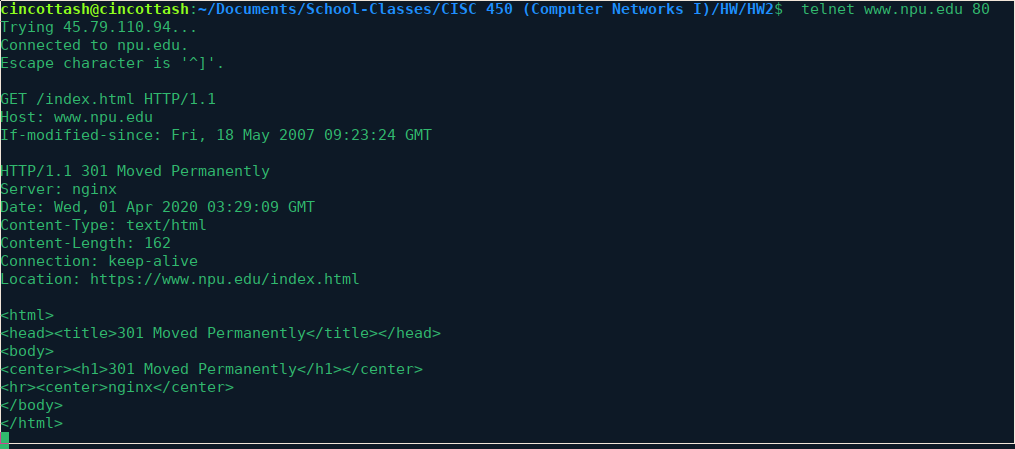
\includegraphics[scale=0.45]{RQ14.png}
\caption{}
\end{figure}


\section{Chapter 2, Review Question 15}
SMS can use one or more protocols, some of them include: TPC, HTTP, HTTPS, FPT.\\
\newline Some popular messaging apps and their protocols include : Vibe-TCP, Skype-VoIP, Facebook Messenger-XMPP, Yahoo Messenger-TCP/HTTP.\\
\newline Thus some messaging apps can use the same protocols, while some use different protocols.\\


\section{Chapter 2, Review Question 20}
\begin{figure}[h!]
\centering
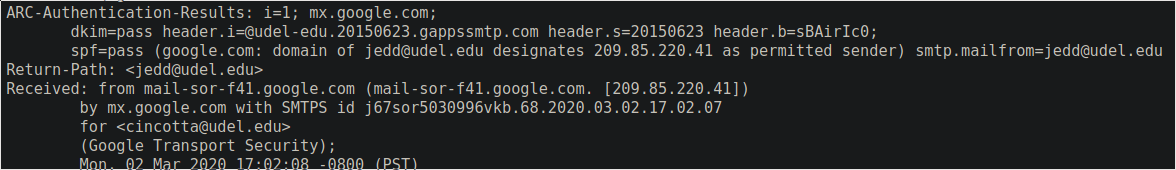
\includegraphics[scale=0.65]{RQ20a.png}
\caption{}
\end{figure}
Figure 2 shows the header from an email I received from a .edu email address.  You can see the IP address of the host from which the message was sent.\\

The IP address of the sender's host is only included in the Received: hedaer line if the mail is sent from an SMTP environment.  Gmail uses a non-SMTP environment, thus the IP address of the senders host is not included in the Received field.\\

\section{Chapter 2, Review Question 26}
The reason is because TCP is a connection-oriented protocol.  This entails that TCP has a welcoming socket, in addition to the client's socket that is created during a connection.  UDP is a connection-less protocol and as such only has one socket.  This socket is used to send a receive data from the client.  Thus for a TCP server to hold n connections, n+1 sockets are needed.  N is the number of clients connecting, plus 1 more for the welcoming socket.\\

\section{Chapter 2, Review Question 27}
TCP is a connection-oriented protocol, this means that a connection between the server and client must be established before data can be transferred.  A connection request must first be accepted by a socket on the TCP server.  Thus in order for this listening socket to exist and accept connections, the server must start before the client connects.  UDP is a connection-less protocol, this entails that a connection does not need to be established before attempting to send data.  UDP also permits packets to be lost, that is, if a sent packet fails to reach it's endpoint, it will not be resent.\\

\section{Chapter 2, Problem 1}
\subsection{a}
False, In HTTP, the client must send one request per object.\\
\subsection{b}
True, because the exist on the same domain.\\
\subsection{c}
False, a TCP segment can only carry multiple HTTP request message with a persistent connection.\\
\subsection{d}
False, the Date: header indicates the time and date when the object in the response was created and sent by the server.\\
\subsection{e}
False, the server may send an empty body along with a status code such as 400, 404 if the requested file is unable to be found.\\

\section{Chapter 2, Problem 3}
In the transport layer, UDP is needed for DNS, and TCP is needed for HTTP.\\
\newline  In the application layer, DNS and HTTP are needed.\\

\section{Chapter 2, Problem 5}
\begin{figure}[h!]
\centering
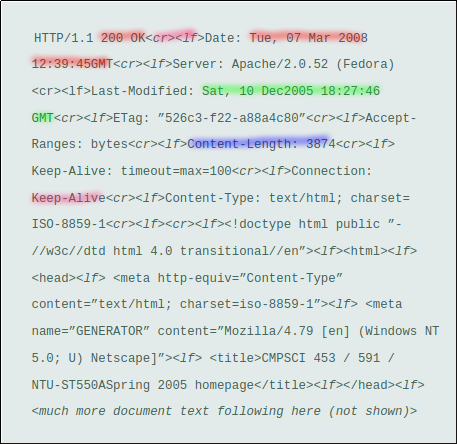
\includegraphics[scale=0.65]{Q5.png}
\caption{}
\end{figure}

\subsection{a}
The server was able to find the document.  The reply was provided at Tue, 07 Mar 2008 12:39:45GMT.\\
\newline I found the answer in the red highlighted section of figure 3.\\

\subsection{b}
The document was last modified Sat, 10 Dec 2005 18:27:46 GMT.\\
\newline I found the answer in the green highlighted section of figure 3.\\

\subsection{c}
3874 bytes are in the doucment being returned.\\
\newline I found the answer in the blue highlighted section of figure 3.\\

\subsection{d}
The first 5 bytes are $<$!doc.  THe server agreed to a persistent connection.\\
\newline I found the answer in the pink highlighted section of figure 3.\\

\section{Chapter 2, Problem 6}
\subsection{a}
According to the the HTTP/1.1 specification (RFC 2616), a client, server or both can send the close of connection signal.  To close the connection, the connection header field is sent Connection token close.\\

\subsection{b}
The HTTP/1.1 specification (RFC 2616) does not provide encryption services.\\

\subsection{c}
According to section 8.14 of RFC-2616, the number of connections that a client have have simultaneously with a server or proxy is 2.\\

\subsection{d}
Yes this is possible.  The transport connection can be closed from either the client or server side at any time.  The server may initiate a signal to close a connection after that connection has been idle for some amount of time.  At the same time, the client can send a request to the server (via the same connection), but the client is unaware of the asynchronous closing of the connection.\\

\section{Chapter 2, Problem 7}
The amount of time that elapses from when a user clicks the link until the object is received by the client is: Time for DNS lookup + Time to establish TPC connection + Time to send request/receive object.\\
\newline = $2RTT_0 + (RTT_1 + RTT_2 + RTT_n)$\\

\section{Chapter 2, Problem 8}
\subsection{a}
THe time to receive an object by the client is: Time to establish TCP connection + time to send the request/receive object + transmission time of object.\\
\newline = $2RTT_0$ = $16RTT_0$ (multiplied by 8 for the 8 objects).\\
\newline Thus the total time taken for DNS lookup + time to establish TCP connection + time to send request/receive object + time to receive 8 objects.\\
\newline = $18RTT_0 + (RTT_1 + RTT_2 + RTT_n)$\\

\subsection{b}
The time to establish a TCP connection + time to request/receive an object is $2RTT_0$.\\
\newline Thus the total time that elapses from when a user clicks the link until the file is receive by the client is time taken for DNS + time to establish TCP connection + time to send request/receive reply + time to receive 8 objects.\\
\newline = $4RTT_0 + (RTT_1 + RTT_2 + RTT_n)$\\

\subsection{c}
Because of persistence, the 8 objects can be received in one RTT.\\
Thus the total time taken for DNS lookup + time to establish TCP connection + time to send request/receive object + time to receive 8 objects.\\
\newline = $3RTT_0 + (RTT_1 + RTT_2 + RTT_n)$\\

\section{Chapter 2, Problem 9}
\subsection{a}
The average time = $\frac{L}{R} = \frac{850k bits}{15M bits/sec} = 0.0567$ seconds.\\
\newline The average access delay = $\frac{0.0567}{1- (16 * 0.0567)}$ = 0.61099 seconds.\\
\newline The total average time is determined with the following formula:\\
\newline Total Average Time = Average access delay + average internet delay = $0.061099 + 3$ = 3.61099 seconds.\\

\subsection{b}
With a miss ratio of 0.4, the average access delay becomes $\frac{0.0567}{1- (0.4) * 0.9072}$ = 0.089 seconds.\\
\newline Thus the average response time is 0.089 + 3 = 3.089 seconds.\\
\newline Thus the total response time is $0.4 * 3.089 sec$ = 1.24 seconds.\\

\section{Chapter 2, Problem 20}
To do this, one would simply need to look at the requests in the cache to different web servers at different points in time.  After collection enough data (essentially snapshots of what is in the cache at what time), one could then could make a graph of the frequency distribution of web servers recorded by the cache of the DNS server.  The servers with the highest frequency are the most popular web servers among the users of the department.\\

\end{document}